% The VLA control loop, drawn in the same TikZ style as the pipeline figure
% (assets/pipeline.tex) so the two diagrams read as one family.
% Build: pdflatex vla_loop.tex && pdftocairo -svg vla_loop.pdf ../public/figs/vla_loop.svg
\documentclass[tikz,border=4pt]{standalone}
\usepackage{amsmath,amssymb}
\usetikzlibrary{arrows.meta,positioning,calc,fit,backgrounds,shapes.geometric}

\begin{document}
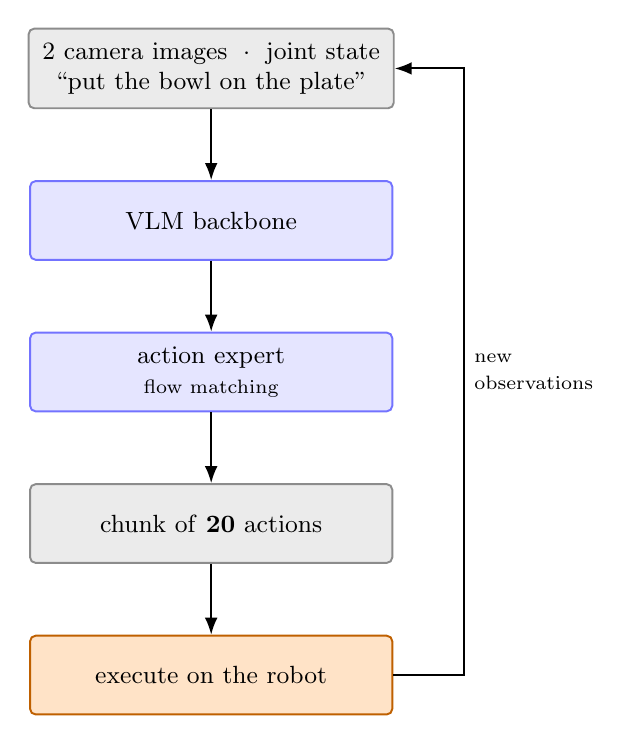
\begin{tikzpicture}[font=\small, >=Latex, line width=0.7pt, node distance=9mm,
  box/.style={draw, rounded corners=2pt, align=center, inner sep=5pt,
              minimum height=10mm, minimum width=46mm},
  data/.style={box, fill=black!8,   draw=black!45},
  pol/.style={box,  fill=blue!10,   draw=blue!55},
  act/.style={box,  fill=orange!22, draw=orange!75!black}]

\node[data] (obs)   {2 camera images $\;\cdot\;$ joint state\\
                     ``put the bowl on the plate''};
\node[pol]  (vlm)   [below=of obs]  {VLM backbone};
\node[pol]  (exp)   [below=of vlm]  {action expert\\{\scriptsize flow matching}};
\node[data] (chunk) [below=of exp]  {chunk of \textbf{20} actions};
\node[act]  (rob)   [below=of chunk] {execute on the robot};

\draw[->] (obs)   -- (vlm);
\draw[->] (vlm)   -- (exp);
\draw[->] (exp)   -- (chunk);
\draw[->] (chunk) -- (rob);

% closed loop: only between chunks, never within one
\draw[->] (rob.east) -- ++(9mm,0) |- node[right, pos=0.25, align=left]
  {\scriptsize new\\[-1pt]\scriptsize observations} (obs.east);

\end{tikzpicture}
\end{document}
